\documentclass{iopjournal}

\usepackage{amsmath,amssymb,bm}
\usepackage{booktabs}
\usepackage{tabularx}
\usepackage[authoryear,round]{natbib}
\usepackage{xcolor}
\usepackage{float} % Fixed placement for the requested figure/table pages.

\newcommand{\ones}{\bm{1}}
\newcommand{\Dmat}{\bm{D}}
\newcommand{\rvec}{\bm{r}}
\newcommand{\revisionpending}{\textcolor{red}{\textbf{GPU result pending}}}
\providecommand{\revstart}{}
\providecommand{\revstop}{}
% Generated by scripts/materialize_revision_assets.py; do not edit.
\newcommand{\RevisionAnalysisStatus}{complete}
\newcommand{\SimulationDasWidth}{0.2255}
\newcommand{\ExperimentalDasWidth}{0.5732}
\newcommand{\CarotidCcDasGcnr}{0.734}
\newcommand{\CarotidClDasGcnr}{0.950}
\newcommand{\KernelDasTime}{0.073}
\newcommand{\SimulationCfWidth}{0.1459}
\newcommand{\ExperimentalCfWidth}{0.4212}
\newcommand{\CarotidCcCfGcnr}{0.938}
\newcommand{\CarotidClCfGcnr}{0.818}
\newcommand{\KernelCfTime}{6.395}
\newcommand{\SimulationMvWidth}{0.1743}
\newcommand{\ExperimentalMvWidth}{0.4132}
\newcommand{\CarotidCcMvGcnr}{0.734}
\newcommand{\CarotidClMvGcnr}{0.964}
\newcommand{\KernelMvTime}{416.692}
\newcommand{\SimulationDmasWidth}{0.3706}
\newcommand{\ExperimentalDmasWidth}{0.3496}
\newcommand{\CarotidCcDmasGcnr}{0.754}
\newcommand{\CarotidClDmasGcnr}{0.962}
\newcommand{\KernelDmasTime}{4.175}
\newcommand{\SimulationReceiveNsiWidth}{0.0090}
\newcommand{\ExperimentalReceiveNsiWidth}{0.0638}
\newcommand{\CarotidCcReceiveNsiGcnr}{0.458}
\newcommand{\CarotidClReceiveNsiGcnr}{0.596}
\newcommand{\KernelReceiveNsiTime}{0.737}
\newcommand{\SimulationAngleNsiWidth}{0.1160}
\newcommand{\ExperimentalAngleNsiWidth}{0.0713}
\newcommand{\CarotidCcAngleNsiGcnr}{0.448}
\newcommand{\CarotidClAngleNsiGcnr}{0.594}
\newcommand{\KernelAngleNsiTime}{0.372}
\newcommand{\EndToEndDasTime}{22.66}
\newcommand{\MbtraceDasWidth}{0.286}
\newcommand{\MbtraceDasMatch}{100.0}
\newcommand{\EndToEndReceiveNsiTime}{27.03}
\newcommand{\MbtraceReceiveNsiWidth}{0.111}
\newcommand{\MbtraceReceiveNsiMatch}{83.3}
\newcommand{\EndToEndAngleNsiTime}{23.86}
\newcommand{\MbtraceAngleNsiWidth}{0.184}
\newcommand{\MbtraceAngleNsiMatch}{50.0}
\newcommand{\PicmusReceiveNsiNotchCount}{4}
\newcommand{\PicmusAngleNsiNotchCount}{3}

\pdfstringdefDisableCommands{\def\revstart{}\def\revstop{}}

\ifdefined\revisionhighlight
\fancyhead[L]{{\color{black}\small\sf IOP Publishing}\hspace{5mm}
{\color{black}\it Phys. Med. Biol.} {\color{black}\bf vv}
{\color{black}(yyyy) aaaaaa}}
\fancyhead[R]{{\color{black}Leroy}}
\fancyfoot[C]{{\color{black}\thepage}}
\fi

\begin{document}

\articletype{Note}

\title{Angle-domain null subtraction imaging from beamformed plane-wave data}

\author{Henri Leroy$^{1,*}$\orcid{0009-0009-7215-6796}}

\affil{$^1$Laboratory of Wave Engineering, School of Engineering, Ecole
Polytechnique Federale de Lausanne (EPFL), Lausanne, Switzerland}

\affil{$^*$Author to whom correspondence should be addressed.}

\email{henri.leroy@epfl.ch}

\keywords{ultrafast ultrasound, plane-wave imaging, null subtraction imaging,
angular apodization, beamforming}

\begin{abstract}
\textit{Objective.} Null subtraction imaging (NSI) narrows the apparent lateral
response by combining fields produced with a zero-mean apodization and two
DC-offset variants. \revstart Usually, NSI requires channel data and flexible beamformers (Receive-NSI). We investigate Angle-NSI, \revstop which operates on per-angle images during coherent plane-wave compounding.

\textit{Approach.} A matrix formulation was used to distinguish receive-domain
and angle-domain null subtraction expressions and to identify their independent
computational components. \revstart A small-angle model gives a physical
interpretation of the angular null.\revstop{} The method was evaluated using a
simulated point target, \revstart experimental resolution phantom targets,\revstop{} an open microbubble (MB) traces dataset and two
\textit{in vivo} carotid acquisitions. Angle sampling, noise, phase jitter and target position were swept in
simulation. A synchronized GPU benchmark compared the complete reconstructions. \revstart Six beamforming methods were compared:
delay-and-sum (DAS), coherence-factor-weighted DAS (CF-DAS), minimum variance beamforming
(MV), delay-multiply-and-sum (DMAS), Receive-NSI and Angle-NSI.\revstop{}

\textit{Main results.} \revstart Angle-NSI \revstop reduced the simulated $-6$ dB lateral width
from 0.226 mm for DAS to 0.116 mm,
compared with 0.009 mm for \revstart Receive-NSI\revstop, while the axial width was 0.720 mm for these three methods. \revstart The lateral narrowing was confirmed on an experimental resolution phantom. Angle-NSI had shorter reconstruction time than Receive-NSI and the lowest post-delay processing time among the nonlinear methods. \revstop In power Doppler, microbubble trace widths were reduced by 50.2\% for conventional NSI and 30.9\% for angular NSI compared to DAS. \revstart On a phantom and \revstop \textit{in vivo}, both NSI variants reduced generalized contrast-to-noise ratio relative to \revstart the
conventional methods\revstop.

\textit{Significance.} \revstart Angle-NSI provides simple post-processing of per-angle beamformed images. It narrows the apparent lateral response at low computational cost, at the expense of B-mode detectability: this makes it a well-suited alternative for high-resolution power Doppler applications. \revstop 
\end{abstract}

\vspace{0.2cm}
\noindent{\small \textbf{Word counts:} Manuscript: 3499 words,
including the abstract and figure/table captions but excluding references;
Abstract: 275 words.}
\par\medskip

\section{Introduction}

Coherent plane-wave compounding combines images acquired after a sequence of
steered, unfocused transmissions and is central to modern ultrafast ultrasound
\citep{montaldo2009coherent,tanter2014ultrafast}. Its high acquisition rate
supports many applications, but conventional delay-and-sum (DAS)
\revstart lateral\revstop{} resolution remains set by the transmit and receive
apertures.

Null subtraction imaging (NSI) is a nonlinear alternative that exploits the
sharp spatial variation around a beam-pattern null. A zero-mean receive
apodization and two DC-offset variants are applied to the same channel data;
their envelopes are then combined incoherently. Because these apodizations act
across the receive aperture, the original method was introduced to narrow the
apparent lateral point-spread function (PSF) \citep{reeg_improving_2015,agarwal2019improving}. It has therefore been used for
high-resolution imaging and grating-lobe suppression
\citep{kou2022grating,gardner2024gratinglobe,kou_detection_2023,
kou2024highresolution}. Sensitivity, contrast and speckle preservation
nevertheless depend on the offset, noise and target properties
\citep{agarwal2019improving,kou2024highresolution}. Recent adaptive variants
have consequently focused on the trade-off between resolution and image quality
\citep{xu2026regionadaptive,yang2026generalized} and on translation to
low-frequency imaging \citep{xu_frame_2024,xu_null_2025}.

\revstart Receive-NSI\revstop{} is naturally less convenient than standard
plane-wave compounding in software pipelines that expose only beamformed images
or do not support custom element weights
\citep{garcia2021must,guan_mach_2026}. Angular apodization offers another degree
of freedom: the per-angle complex images may themselves be weighted before
compounding \citep{rodriguez-molares_angular_2015}. This suggests translating
the NSI null from receive elements to steering angles. Such a construction is
computationally light once the angle stack is available, and the two
constructions are algebraically distinct because their weights act on different
axes of the data.

\revstart This Note compares Angle-NSI with DAS, CF-DAS, MV, DMAS and Receive-NSI using simulation, an experimental phantom, microbubble power Doppler and carotid B-mode imaging. It provides a post-processing technique for beamforming pipelines retaining per-angle images without RF data access. \revstop

\section{Methods}

\subsection{Receive-domain and angle-domain null fields}

Consider an ultrafast imaging sequence using $N_\theta$ plane waves and $N_e$
receive elements. At an image point $\rvec=(x,z)$, collect the complex data
sampled at the predicted transmit--receive time of flight in
$\Dmat(\rvec)\in\mathbb{C}^{N_\theta\times N_e}$, with:
\begin{equation}
D_{kn}(\rvec)=s_k^n\!\left(\tau_{kn}(\rvec)\right)
\end{equation}
where $s_k^n(t)$ is the demodulated signal recorded by element $n$ after
transmission $k$, and $\tau_{kn}(\rvec)$ is the corresponding
transmit--receive time of flight.

Let $\bm{w}=(w_1,\ldots,w_{N_e})^{\mathrm T}\in\mathbb{R}^{N_e}$ denote the
receive-apodization vector, and let $\ones_\theta\in\mathbb{R}^{N_\theta}$
denote the column vector of equal weights used for coherent compounding across
the transmitted plane waves. The resulting complex DAS field is:
\begin{equation}
U(\rvec)=\ones_\theta^{\mathrm T}\Dmat(\rvec)\bm{w}
=\sum_{k=1}^{N_\theta}\sum_{n=1}^{N_e}w_nD_{kn}(\rvec)
\label{eq:uniform}
\end{equation}
\revstart For uniform receive apodization, $\boldsymbol{w}=\boldsymbol{1}_e$, where $\boldsymbol{1}_e\in\mathbb{R}^{N_e}$ is the all-ones column vector. Thus, $U(\boldsymbol{r})$ is the summed reference DAS field, with envelope $|U(\boldsymbol{r})|$. \revstop

NSI is formed using a beam-pattern null produced via a zero-sum apodization; two
companion signals are then obtained by adding the same uniform DC offset to this
apodization and to its sign-reversed counterpart, and the null-field envelope
is subtracted from the mean of their envelopes
\citep{agarwal2019improving}. To express NSI, let $Z$ denote \revstart the null field generated by an apodization whose coefficients sum to zero\revstop, and let $c>0$ be the DC offset. Because the two offset fields are $Z+cU$ and
$-Z+cU$, the NSI envelope can be written as the functional:
\begin{equation}
\mathcal{N}(U,Z;c)=\frac{|Z+cU|+|-Z+cU|}{2}-|Z|
\label{eq:functional}
\end{equation}

For \revstart Receive-NSI\revstop, the null component is formed using a
receive-apodization vector $\bm{w}_{\mathrm{null}}\in\mathbb{R}^{N_e}$ whose
coefficients sum to zero, $\ones_e^{\mathrm T}\bm{w}_{\mathrm{null}}=0$, and
have opposite signs on the two halves of the active receive aperture. The two
offset receive apodizations are consequently
$\bm{w}_{\pm}=\pm\bm{w}_{\mathrm{null}}+c\ones_e$. The receive-domain null field
and NSI envelope are:
\begin{equation}
Z_e(\rvec)=\ones_\theta^{\mathrm T}\Dmat(\rvec)\bm{w}_{\mathrm{null}},
\qquad E_e(\rvec)=\mathcal{N}\left(U(\rvec),Z_e(\rvec);c\right)
\label{eq:receive}
\end{equation}
With dynamic receive focusing, the active aperture and the position of the sign
transition are updated for each pixel.

Here, we propose an alternative angle-domain construction for NSI. The receive
apodization remains uniform, while the zero-sum sign change is applied across
the steering sequence:
\begin{equation}
Z_{\theta}(\rvec)=\bm{v}_{\rm null}^{\mathrm T}\Dmat(\rvec)\ones_e,
\qquad E_\theta(\rvec)=\mathcal{N}\left(U(\rvec),Z_\theta(\rvec);c\right)
\label{eq:angle}
\end{equation}
where $v_{{\rm null},k}=\operatorname{sign}(\theta_k)$ for a symmetric angular
sequence. \revstart The symmetry of the construction of Eq. \eqref{eq:functional} requires positive and negative angles to be paired in the emission sequence, although their
spacing need not be uniform.\revstop{} If a broadside transmission is present, its zero-mean weight is set to zero. \revstart An incomplete or unpaired sequence requires a
specifically designed null. \revstop Similar behavior is expected when the acquisition
and point response are sufficiently symmetric, but finite angular sampling,
aberration, motion and incomplete insonification can make the two responses
diverge. 

\revstart To understand how angular summation affects the response, let \(B_k\) denote the complex image reconstructed from transmit angle \(\theta_k\). The reference and angular null fields are:
\begin{equation}
U=\sum_k B_k,\qquad Z_\theta=\sum_k v_{{\rm null},k}B_k
\label{eq:fields-model}
\end{equation}

For a point target located at \(x_0\), consider the beamformed response at \(x=x_0+\Delta x\). Assume matched complex amplitudes \(A_\theta\) within each \(\pm\theta\) pair. With a wavenumber $k_0=2\pi/\lambda_0$, one can write:
\begin{equation}
B_{\pm\theta}(\Delta x)\simeq
A_\theta\exp(\mp\mathrm{i}k_0\Delta x\sin\theta)
\label{eq:paired-angle-model}
\end{equation}

Summing the paired contributions gives:
\begin{equation}
U(\Delta x)\simeq B_0(\Delta x)
+2\sum_{\theta>0}A_\theta\cos(k_0\Delta x\sin\theta)
\label{eq:paired-reference-field}
\end{equation}
where $B_0$ denotes the broadside contribution, set to zero
when no broadside transmission is present.

Near the focus, assuming $|k_0\Delta x\sin\theta|\ll1$ and small transmit angles ($|\theta|\ll1$, i.e. $\sin\theta\simeq\theta$) , one can also write :
\begin{equation}
Z_\theta(\Delta x)\simeq
-2\mathrm{i}k_0\Delta x\sum_{\theta>0}A_\theta\sin\theta \simeq
-2\mathrm{i}k_0\Delta x\sum_{\theta>0}A_\theta\theta
\label{eq:small-angle}
\end{equation}

Using Eq. \eqref{eq:angle}, and writing $S=\sum_{\theta>0}A_\theta\sin\theta$, if the pair amplitudes and broadside contribution share a common phase, this gives:
\begin{equation}
E_\theta(\Delta x)\simeq
\sqrt{c^2|U(\Delta x)|^2+4k_0^2\Delta x^2|S|^2}
-2k_0|\Delta x|\,|S|
\label{eq:angle-local-psf-common-phase}
\end{equation}

In this model, paired contributions cancel in the angular null field at the focus, where $E_\theta(0)=c|U(0)|$. A lateral offset introduces phase shifts of equal magnitude and opposite sign, producing a nonzero angular null field. The resulting Angle-NSI envelope is attenuated relative to $c|U|$ away from the focus, which allows to narrow the apparent lateral response. The null slope depends on angular span, sampling and pair amplitudes, and a broadside component contributes only to \(U\), as shown in Eq. \eqref{eq:paired-reference-field}. Supplementary figure S1 compares paired-angle expression for the angular null with its linear approximation near the focus. \revstop

The angle-domain method is therefore an analogue to \revstart Receive-NSI \revstop that
creates an antisymmetric transmit-angle null while \revstart Receive-NSI\revstop{}
creates the null on receive. 

\subsection{Computational interpretation}

\revstart Angle-NSI and Receive-NSI require two independent
fields, $U$ and $Z$ : 
\begin{itemize}
    \item Receive-NSI forms them from receive-channel samples and a
custom element apodization, which requires at least two complete DAS passes: Kou \textit{et al.} therefore reported a $40\%$ increase in computation time compared to DAS \citep{kou2024highresolution}.
    \item Angle-NSI accumulates $U$ and
$Z_\theta$ from the same per-angle beamformed images before angular compounding. Its incremental cost compared to DAS is consequently low.\revstop
\end{itemize} 

In addition to that, receive-channel samples and a custom element
apodization are not necessarily suited to every beamformer implementation
\citep{garcia2021must,guan_mach_2026}. By contrast, \revstart Angle-NSI \revstop replaces the
unweighted angular sum by two weighted accumulations followed by the envelope
operation in equation~\eqref{eq:functional}. \revstart Its accessibility
advantage applies to research software or scanners that retain per-angle images while keeping RF processing fixed.\revstop

Table~\ref{tab:cost}
summarizes the resulting distinction.

\begin{table}[h!]
\caption{Analysis of processing operations needed after a standard plane-wave
acquisition. ``Additional'' is relative to retaining the usual DAS beamforming and coherent compounding, not counting the final envelope subtraction which applies to both techniques}
\label{tab:cost}
\centering
\begin{tabularx}{\textwidth}{@{}lXX@{}}
\toprule
 & Receive-NSI & Angle-NSI \\
\midrule
Minimal required data & Channel data & Per-angle beamformed images \\
Additional operation & DAS pass & Weights for coherent summation \\
Custom apodization beamformer & Required & Not required \\
\bottomrule
\end{tabularx}
\end{table}

\subsection{\revstart Comparison with other beamforming methods \revstop}
\revstart In addition to DAS and Receive-NSI, Angle-NSI was compared to several nonlinear beamforming methods, such as coherence-factor-weighted DAS, minimum-variance beamforming, and delay-multiply-and-sum:
\begin{itemize}
    \item CF-DAS applied the conventional receive-channel coherence
factor $\mathrm{CF}=\frac{|\sum_m x_m|^2}
{M_{\rm active}\sum_m|x_m|^2}$ to the complex DAS sum for each transmit angle, as described in \citep{li2003adaptive}.
    \item MV used Capon weights, all overlapping subarrays of length
$L=\lfloor M_{\rm active}/2\rfloor$, diagonal loading
$\operatorname{tr}(R)/(100L)$ and axial averaging for carotid data
\citep{synnevag2007adaptive,synnevag2009benefits}. 
    \item DMAS used Matrone's signed
square-root products and a fixed band-pass around $2f_0$ before analytic-envelope
formation \citep{matrone2015delay}. 
\end{itemize}
 
The Python/CuPy implementations were adapted from the corresponding USTB implementations \citep{rodriguez-molares_ultrasound_2017}.
Supplementary section S10 lists all fixed settings.\revstop

\subsection{Data and reconstruction}

Simulations used PyMUST with an L11-5v linear array (128 elements, 0.3 mm pitch
and 7.6 MHz central frequency), 17 plane waves uniformly distributed from
$-4^\circ$ to $4^\circ$, full receive aperture and $c=0.05$
\citep{garcia2021must,bernardino_pymust_2024}. A point scatterer was placed at
$(0,20)$ mm. \revstart The six displayed images used 0.02 mm spatial sampling. Lateral profiles were extracted at each method's peak depth. Receive-NSI, whose
response was narrower than one pixel on the initial grid, was then directly beamformed on a 0.000390625 mm grid, after a dichotomy search to find the first acceptable spatial sampling based on a grid convergence study. Lateral width measurements used linearly interpolated connected $-6$ dB crossings.\revstop

\revstart Experimental PSFs used the public PICMUS
\texttt{resolution\_distorsion} acquisition: 75 angles over
$-16^\circ$--$16^\circ$, 128 elements and seven point targets
\citep{liebgott_plane-wave_2016}. Five targets were near the image axis at
depths from 9.6 to 47.0 mm; two off-axis targets near $\pm10$ mm shared a depth
of approximately 37.5 mm. The image display grid was 0.05 mm laterally
by 0.10 mm axially. Reconstruction grids and display resampling are detailed in supplementary section S10; individual PSF widths, localization errors and peak-to-background levels are reported in section S11. Phantom inclusion
regions are specified in supplementary section S12.\revstop

The \textit{in vitro} evaluation used the public MBTrace data released with
Open-NSI \citep{kou2024highresolution}. The data contain 400 frames acquired
with a 15.625 MHz central frequency, nine steering angles from $-4^\circ$ to
$4^\circ$ and a 128-element array. Reconstruction used a dynamic receive
aperture with F-number 1 and $c=0.1$. A singular-value decomposition (SVD)
clutter filter was applied to the raw images, discarding the first 10 and the
last 50 singular values to visualize flowing microbubbles 
\citep{demene2015spatiotemporal}. Power Doppler was
calculated by integrating the squared magnitude of the filtered signals over slow time \citep{rubin_fractional_1995}.  Peaks were assigned one-to-one to DAS by
minimum distance: \revstart the default tolerance was 0.15 mm, and a
0.05--0.40 mm sweep distinguished peak displacement from absence. Detection required
6 dB prominence, 0.2 mm separation and a level above $-25$ dB after independent
normalization. Only complete three-method (DAS, Receive-NSI, Angle-NSI) triplets were used for paired width
statistics.\revstop

For \textit{in vivo} evaluation, the public PICMUS carotid cross-sectional and
longitudinal channel-data sets were reconstructed on a $128\times250$ grid spanning $x=\pm19.2$ mm and $z=0$--40 mm with a central frequency of 5.21 MHz, 75 emitted angles ranging from
$-16^\circ$ to $16^\circ$, F-number 1, $c=0.05$ and linear interpolation
\citep{liebgott_plane-wave_2016}. Fixed circular lumen and tissue regions of 3 mm radius are shown in
figure~\ref{fig:carotid}. Their $(x,z)$ centers were $(-7.0,15.4)$ and
$(2.0,27.0)$ mm in CL, and $(-1.3,17.7)$ and $(-1.0,27.0)$ mm in CC, for
lumen and tissue, respectively. \revstart Generalized contrast-to-noise ratio (gCNR) was used as the detectability metric, because nonlinear transformations can
alter conventional contrast measures
\citep{rindal2019effect,rodriguez-molares_generalized_2020}.\revstop

\revstart Power-Doppler and B-mode images were normalized method by method for display, and quantitative PSF width measurements used linear envelopes before normalization. The chosen DC offsets for both Receive-NSI and Angle-NSI followed the seminal studies: $c=0.05$ for simulation and PICMUS carotid data, and $c=0.10$ for MBTrace \citep{agarwal2019improving,kou2024highresolution}. \revstop

% Let the simulation figure occupy the top of page 5.
\begin{figure}[!t]
\centering
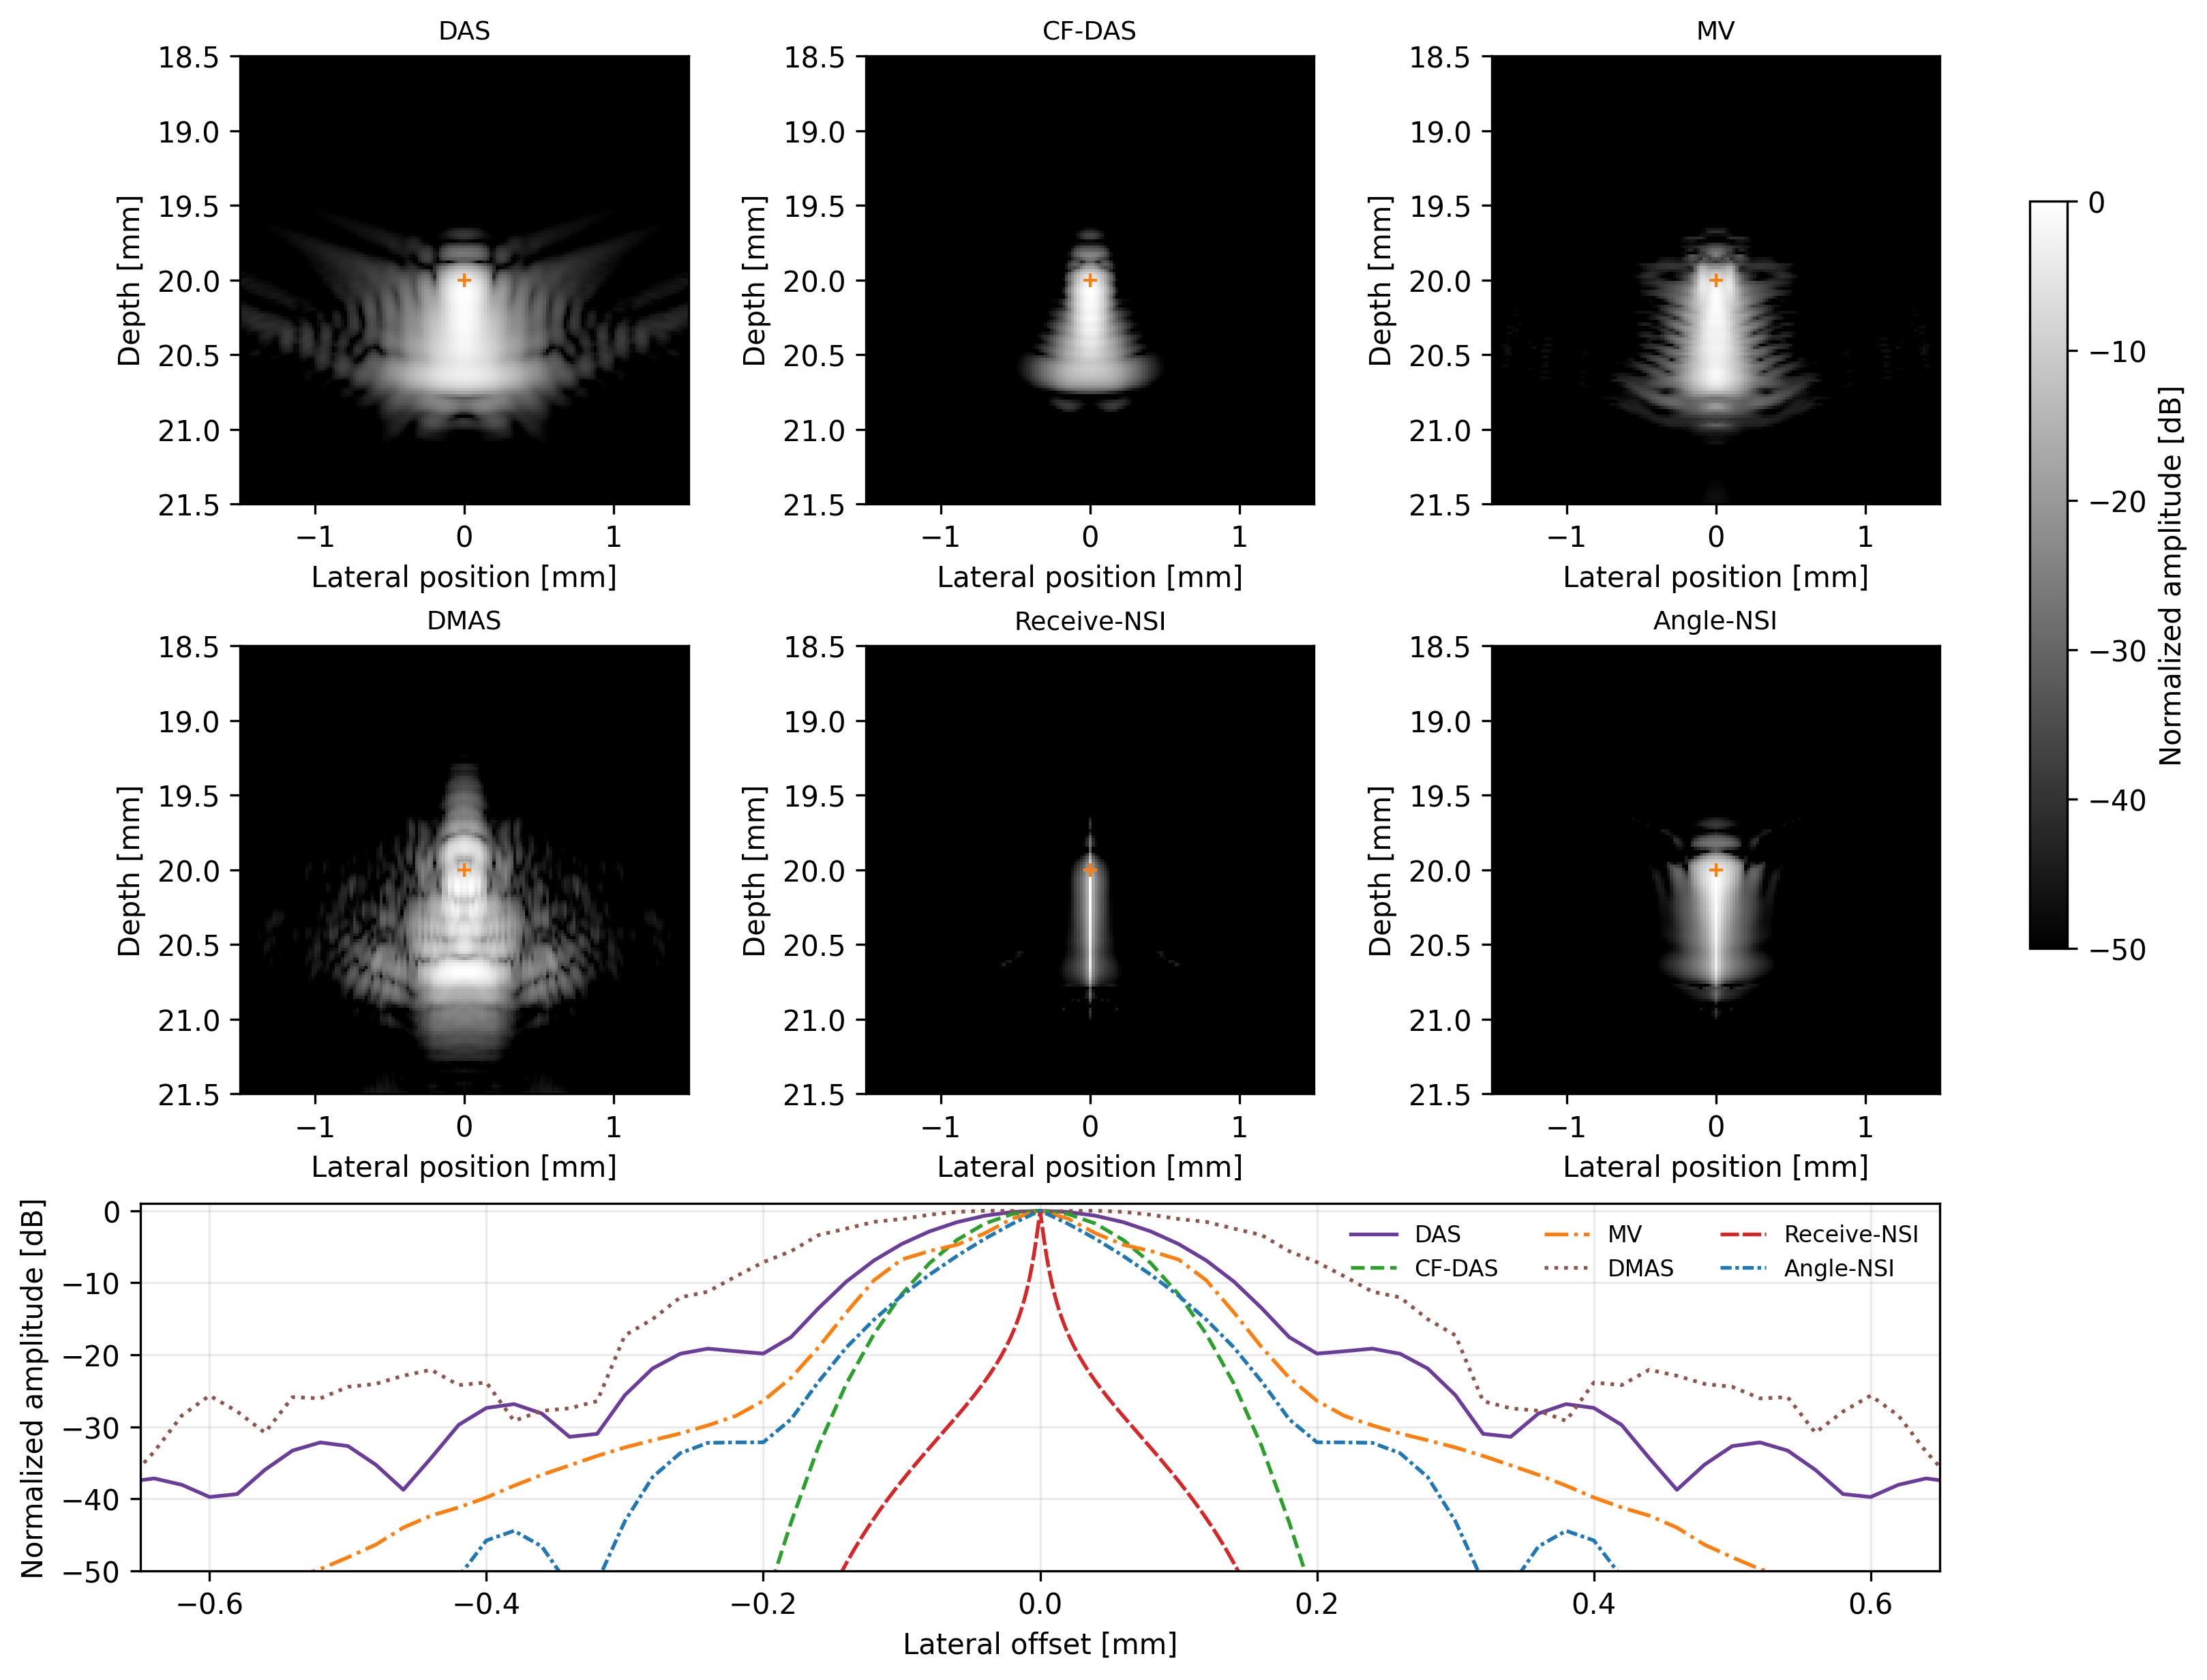
\includegraphics[width=0.9\textwidth]{figures/figure1_simulation_six_method.png}
\caption{\revstart Simulated point-target comparison. The six normalized
envelope maps share a 50 dB display range; the lower panel gives lateral
profiles through each reconstructed peak. Receive-NSI uses its fine-grid
profile. Each method is normalized to its own peak.\revstop}
\label{fig:simulation}
\end{figure}

\subsection{Robustness tests and computation time evaluation}

The point-target model and finest lateral grid were reused for robustness tests.

\revstart \textit{DC offset} : Sensitivity analyses regarding the DC offset used
$c=0.02$, 0.05, 0.10 and 0.20. \revstop

\textit{Dependence on angular sampling}: Counts of 5, 9, 13, 17 and 25 angles were tested over $8^\circ$; spans of $4^\circ$--$16^\circ$ were tested with 17 angles. The $+2^\circ$ transmission was removed using either sign weights or zero-mean recentered weights. 

\textit{Robustness to noise} : Complex noise (40--10 dB SNR) and independent per-angle Gaussian phase offsets (2$^\circ$--20$^\circ$ standard deviation) used ten realizations per level.

\textit{Spatial invariance} : Spatial tests covered four depths and $x=-4$, 0 and 4 mm.


\textit{Timing protocols} : Timing used CuPy 14.1.1 and MACH-beamform 0.1.3 on an RTX A2000 with complex64 IQ data. \revstart Total reconstruction time, including signal focusing and data transfers to and from the GPU, was measured for DAS, Receive-NSI and Angle-NSI. These tests varied image size, receive-element count and plane-wave count. A separate test compared all six methods using signals already focused and stored on the GPU, measuring only the processing needed to combine the focused signals and form an image. Measurements were synchronized with GPU completion. Both tests used ten warm-ups and 50 repetitions per method, and median times were recorded. For the end-to-end tests, repetitions were randomly interleaved and 95\% bootstrap confidence intervals were calculated for the medians. Supplementary section S14 reports additional timing tests assessing the effect of data transfers on reconstruction time. \revstop Acquisition, demodulation, disk input/output and display were excluded.

\section{Results}

\subsection{Point-target response}

The fine-grid reconstruction separated the lateral and axial effects of NSI
(Figure~\ref{fig:simulation}). Angle-NSI reduced the lateral $-6$ dB width from 0.226 mm for DAS to 0.116 mm.
Receive-NSI yielded a lateral width of 0.009 mm,
consistent with earlier reports of very narrow apparent lateral responses
\citep{agarwal2019improving}. \revstart CF-DAS, MV and DMAS gave
\SimulationCfWidth{}, \SimulationMvWidth{} and \SimulationDmasWidth{} mm,
respectively.\revstop{} The axial widths of DAS,
Receive-NSI and Angle-NSI were 0.720 mm, which confirms that NSI sharpens the lateral response without modifying axial resolution \citep{reeg_improving_2015}. 

\revstart Figure~\ref{fig:phantom} represents the experimental responses on the PICMUS phantom.
Table~\ref{tab:comparison} reports the mean $\pm$ sample standard deviation
of lateral $-6$ dB widths and peak-to-background ratios over all seven targets,
together with inclusion gCNR. Both NSI techniques produced narrower lateral
responses and higher peak-to-background ratios than DAS and the other nonlinear beamforming techniques, with lower inclusion
gCNR. Individual PSF measurements and target positions are listed in
supplementary table S7. The NSI responses, however,
varied between targets and sometimes contained secondary lobes.\revstop

\begin{figure}[H]
\centering
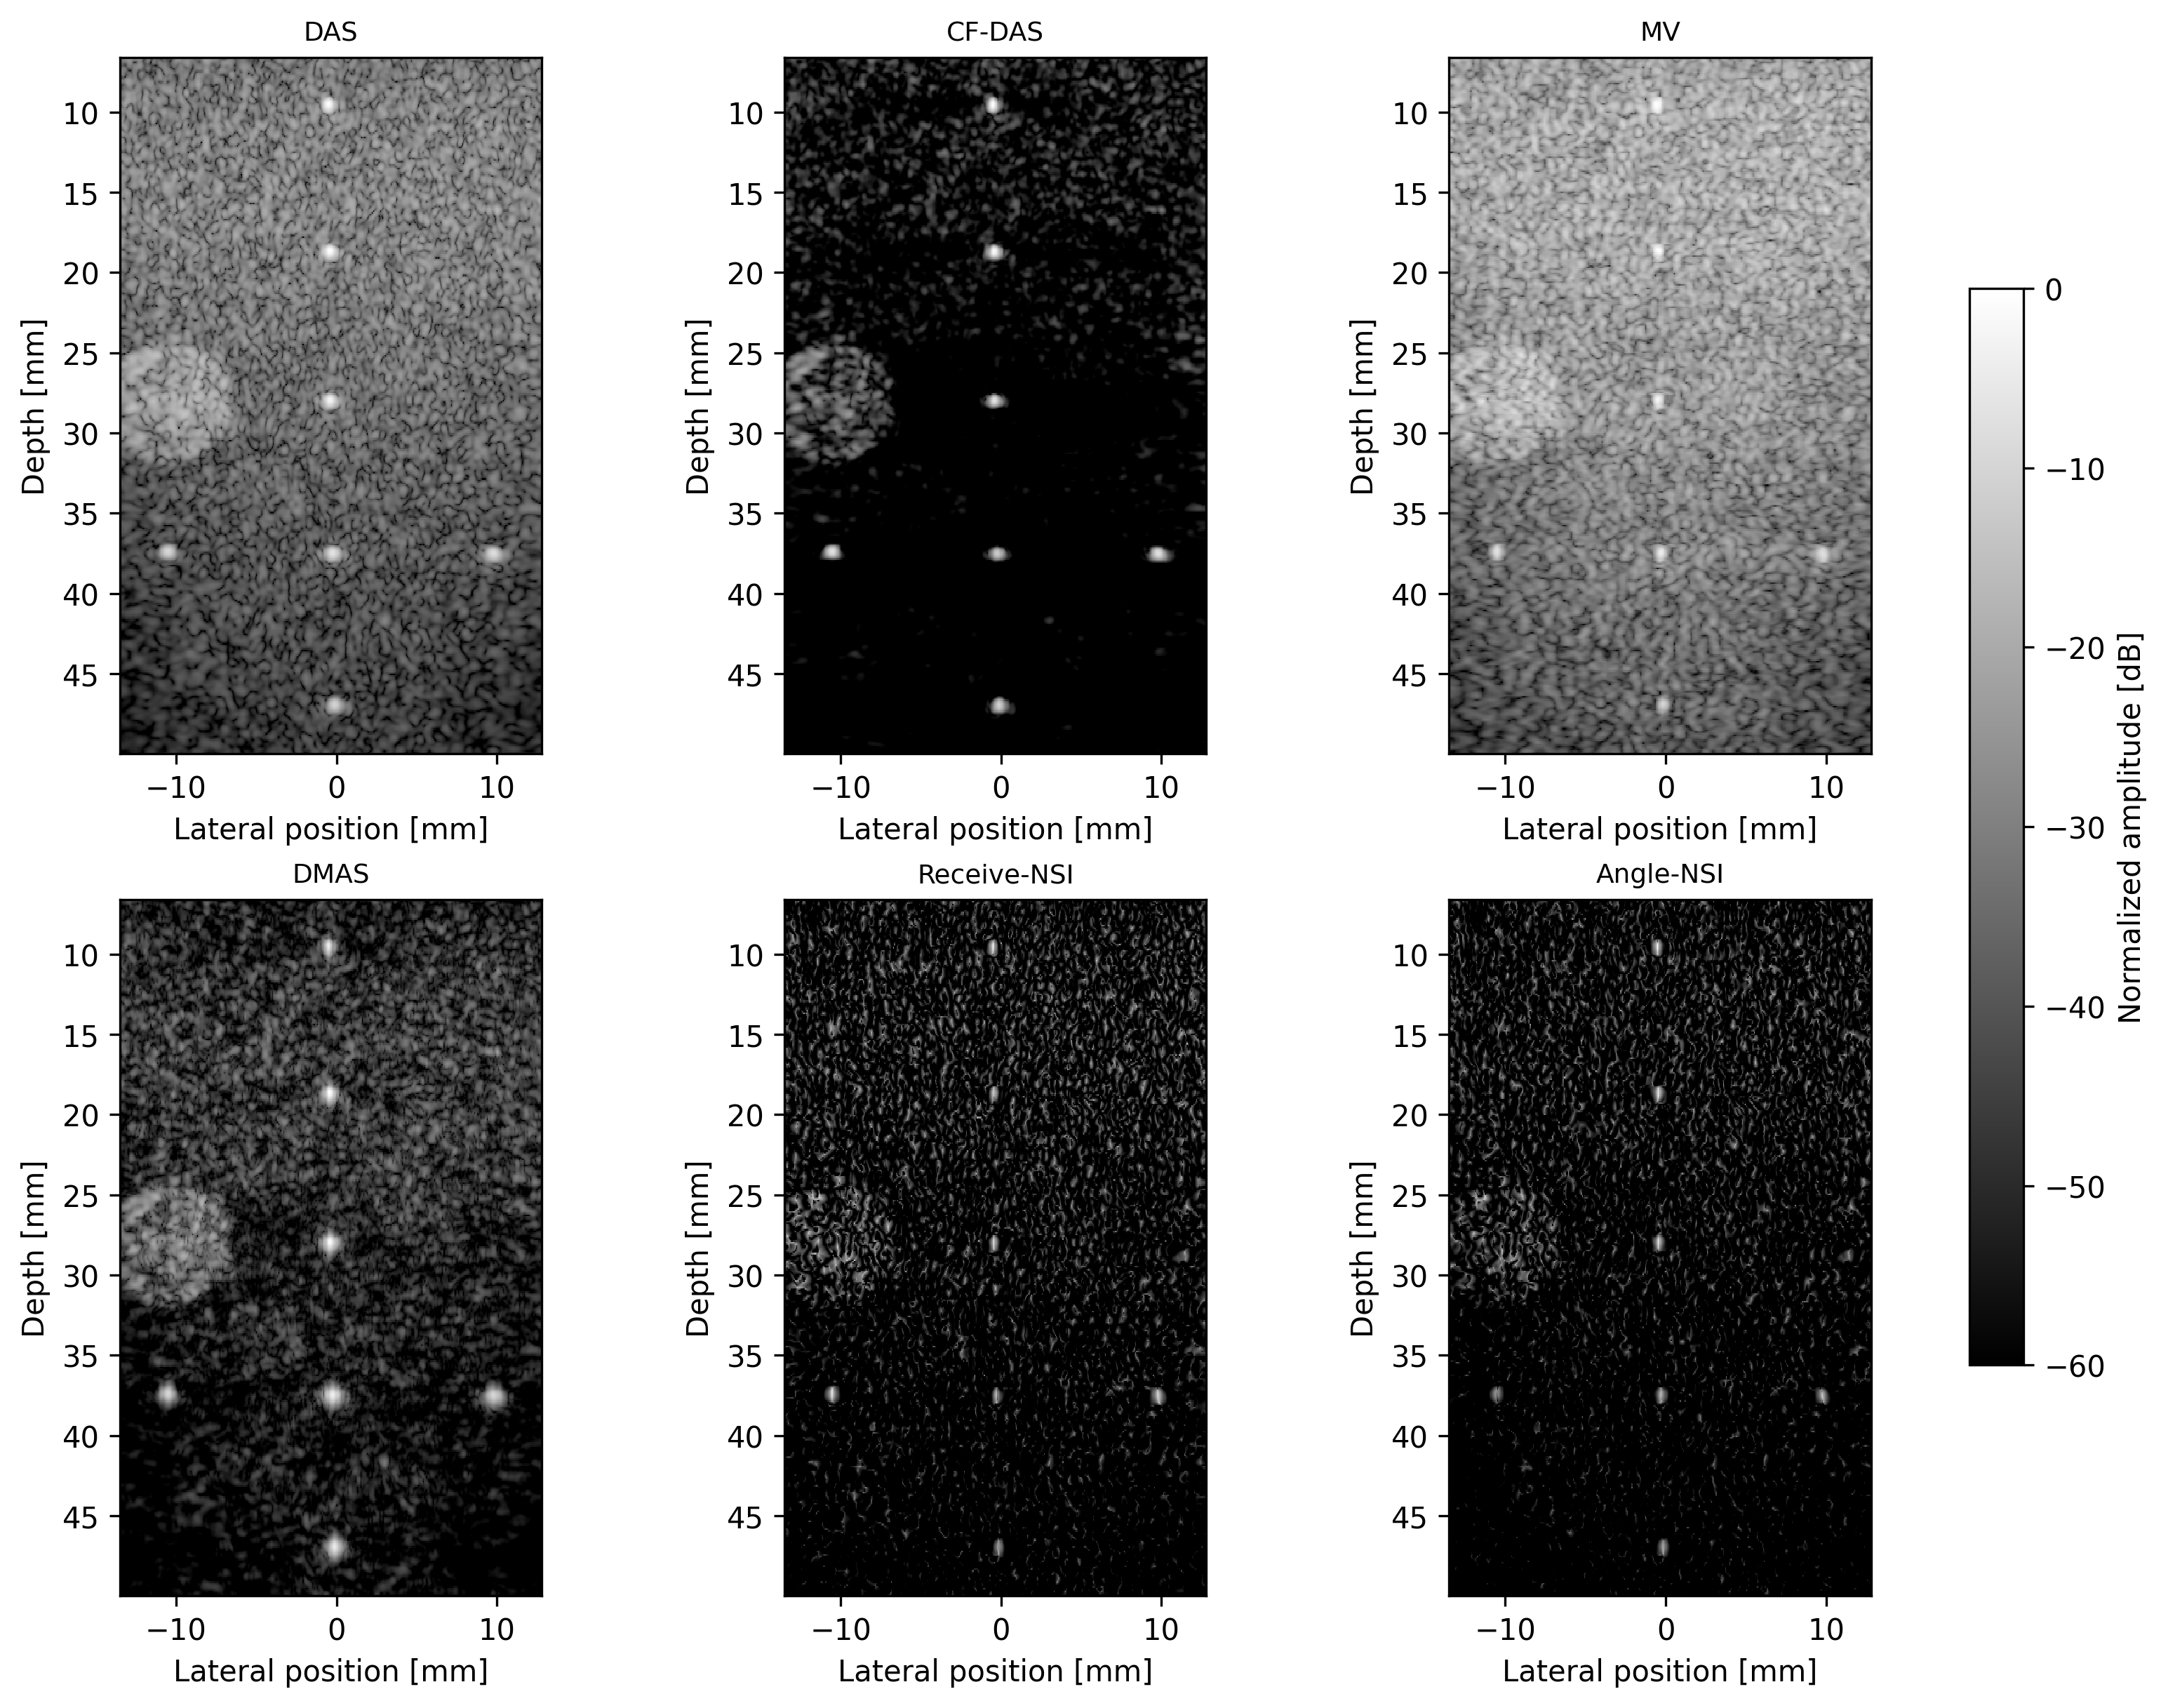
\includegraphics[width=0.85\textwidth]{figures/figure2_picmus_full_phantom_six_method.png}
\caption{\revstart Full experimental PICMUS resolution phantom reconstructed
with the six methods. Each image is normalized to its own peak and displayed
over 60 dB.\revstop}
\label{fig:phantom}
\end{figure}

\begin{table}[H]
\caption{\revstart Experimental PICMUS metrics. Width and peak/background
are mean $\pm$ sample standard deviation over seven point targets (individual
data in supplementary table S7). Inclusion gCNR uses one inclusion/background
region pair at 27.5 mm depth, defined in supplementary section S12.\revstop}
\label{tab:comparison}
\centering
\revstart\begin{tabular}{@{}lrrr@{}}
\toprule
Method & PSF lateral width (mm) & PSF peak/background (dB) & Inclusion gCNR \\
\midrule
DAS & $0.537\pm0.082$ & $26.7\pm1.3$ & 0.732 \\
CF-DAS & $0.391\pm0.074$ & $50.0\pm4.4$ & 0.799 \\
MV & $0.461\pm0.077$ & $23.4\pm4.0$ & 0.620 \\
DMAS & $0.357\pm0.133$ & $32.8\pm3.9$ & 0.769 \\
Receive-NSI & $0.051\pm0.016$ & $57.0\pm3.3$ & 0.299 \\
Angle-NSI & $0.070\pm0.030$ & $55.3\pm4.1$ & 0.285 \\
\bottomrule
\end{tabular}
\revstop
\end{table}

\subsection{Microbubble power Doppler}

Both NSI techniques show sharper traces than DAS,  combined with a slight loss of sensitivity as
some traces in the upper left corner of the images are not retrieved
(Figure~\ref{fig:doppler}). At $z=10.96$ mm, six DAS peaks, six Receive-NSI
peaks and seven Angle-NSI peaks passed the detection criteria. Five of the six
DAS peaks were positionally concordant with Receive-NSI, whereas three
were concordant with Angle-NSI at 0.15 mm tolerance. \revstart Three Angle-NSI peaks unmatched under the strict criterion of 0.15mm were in fact displaced by 0.202, 0.202 and 0.303 mm: all six DAS peaks had an Angle-NSI counterpart within 0.31 mm, and one region showed a possible split.\revstop

Within the three complete triplets, mean $\pm$ sample standard deviation of
lateral width was $0.266\pm0.056$ mm for DAS, $0.133\pm0.038$ mm for
Receive-NSI and $0.184\pm0.103$ mm for Angle-NSI. The complete tolerance curve
and signed displacements are reported in supplementary section S6.

\begin{figure}[H]
\centering
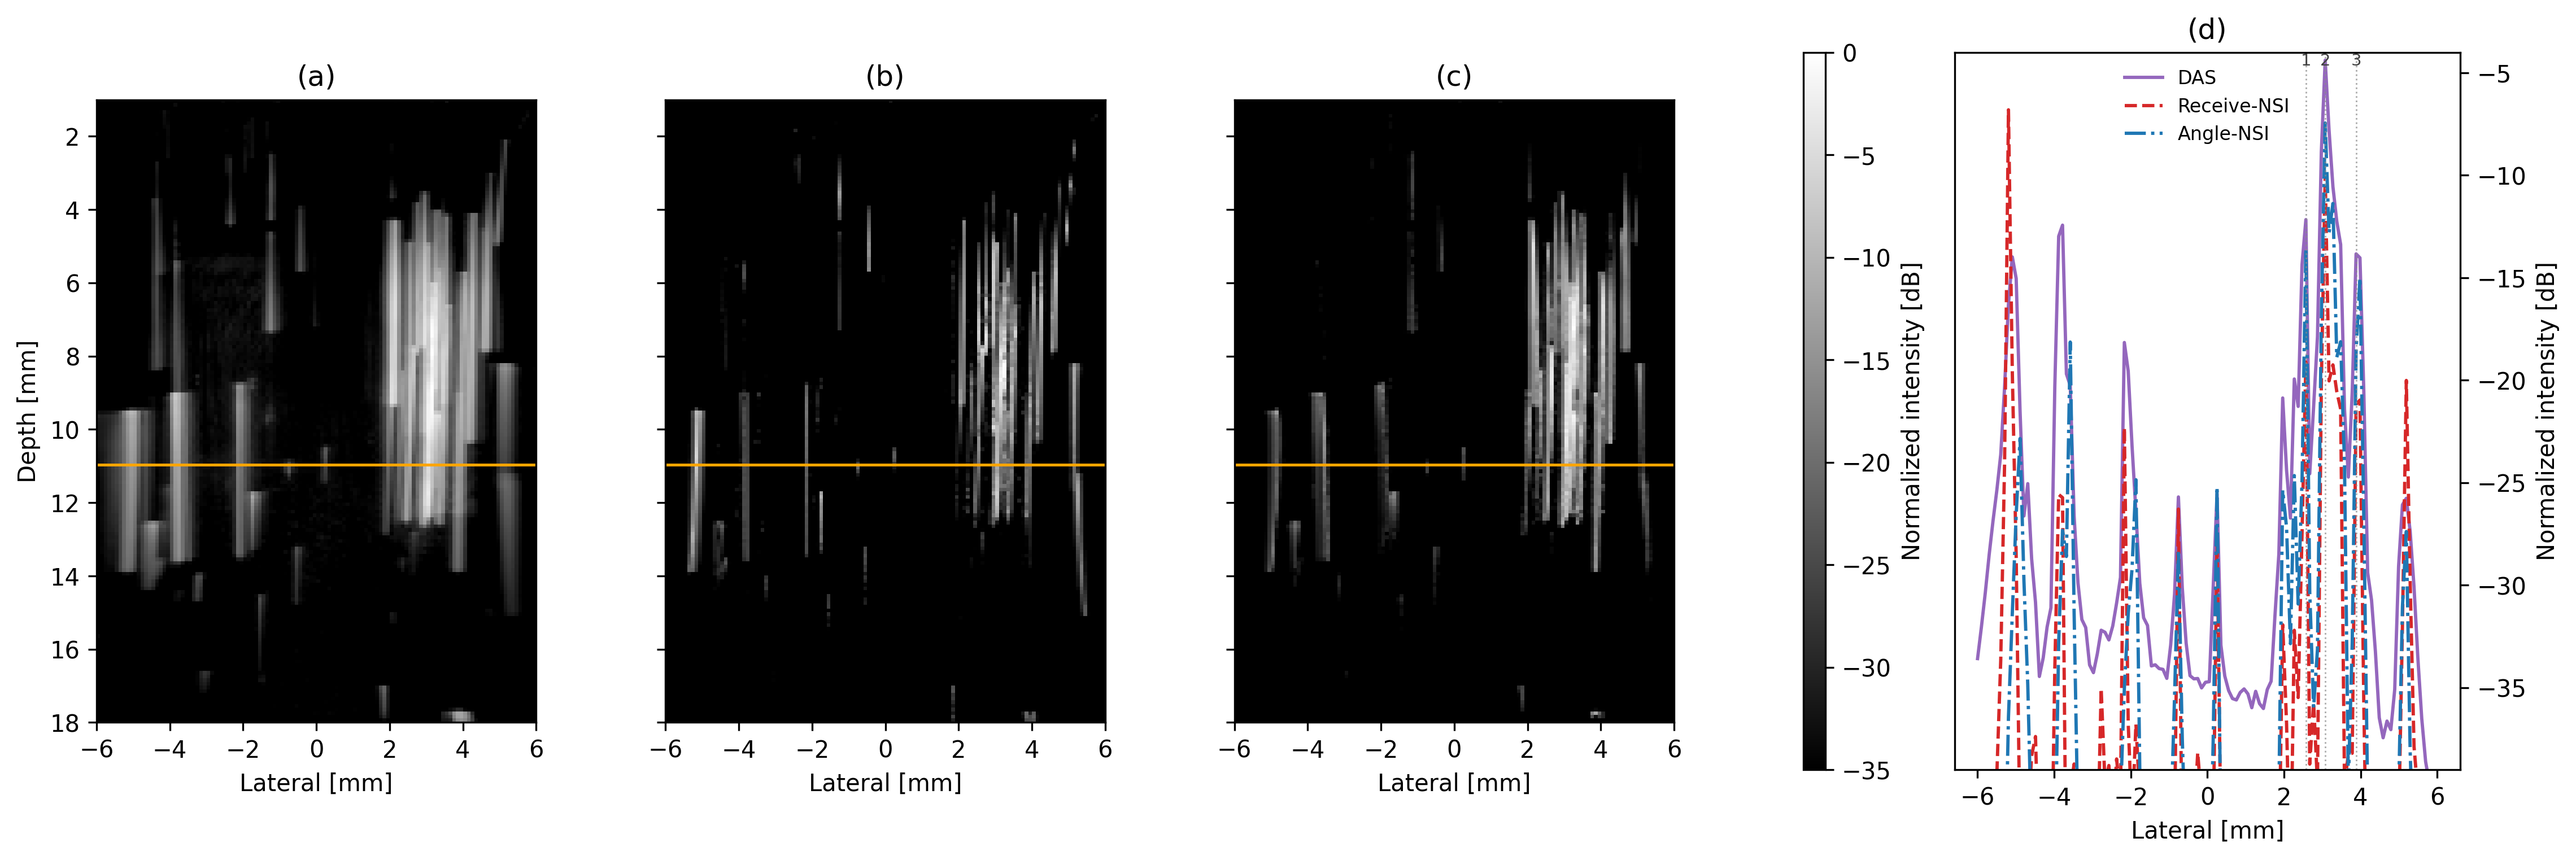
\includegraphics[width=\textwidth]{figures/figure3_microbubble_power_doppler.png}
\caption{\revstart MBTrace power Doppler for (a) DAS, (b) Receive-NSI and
(c) Angle-NSI, with (d) lateral profiles at 10.96 mm. Each method is normalized
to its own maximum and displayed over 35 dB.\revstop}
\label{fig:doppler}
\end{figure}

\subsection{Carotid imaging}

Both NSI variants depicted the carotid lumen but suppressed diffuse speckle
(Figure~\ref{fig:carotid}). \revstart Carotid gCNR values for all six methods
are reported in Table~\ref{tab:carotid-gcnr}. The conventional methods
retained higher gCNR than the NSI methods in
both views: a narrow lateral response and darker background in both NSI variants therefore coexisted with lower tissue-distribution separation, in accordance with earlier observations \citep{agarwal2019improving}. Complete carotid metrics are reported
in supplementary Table S8.\revstop

\begin{figure}[H]
\centering
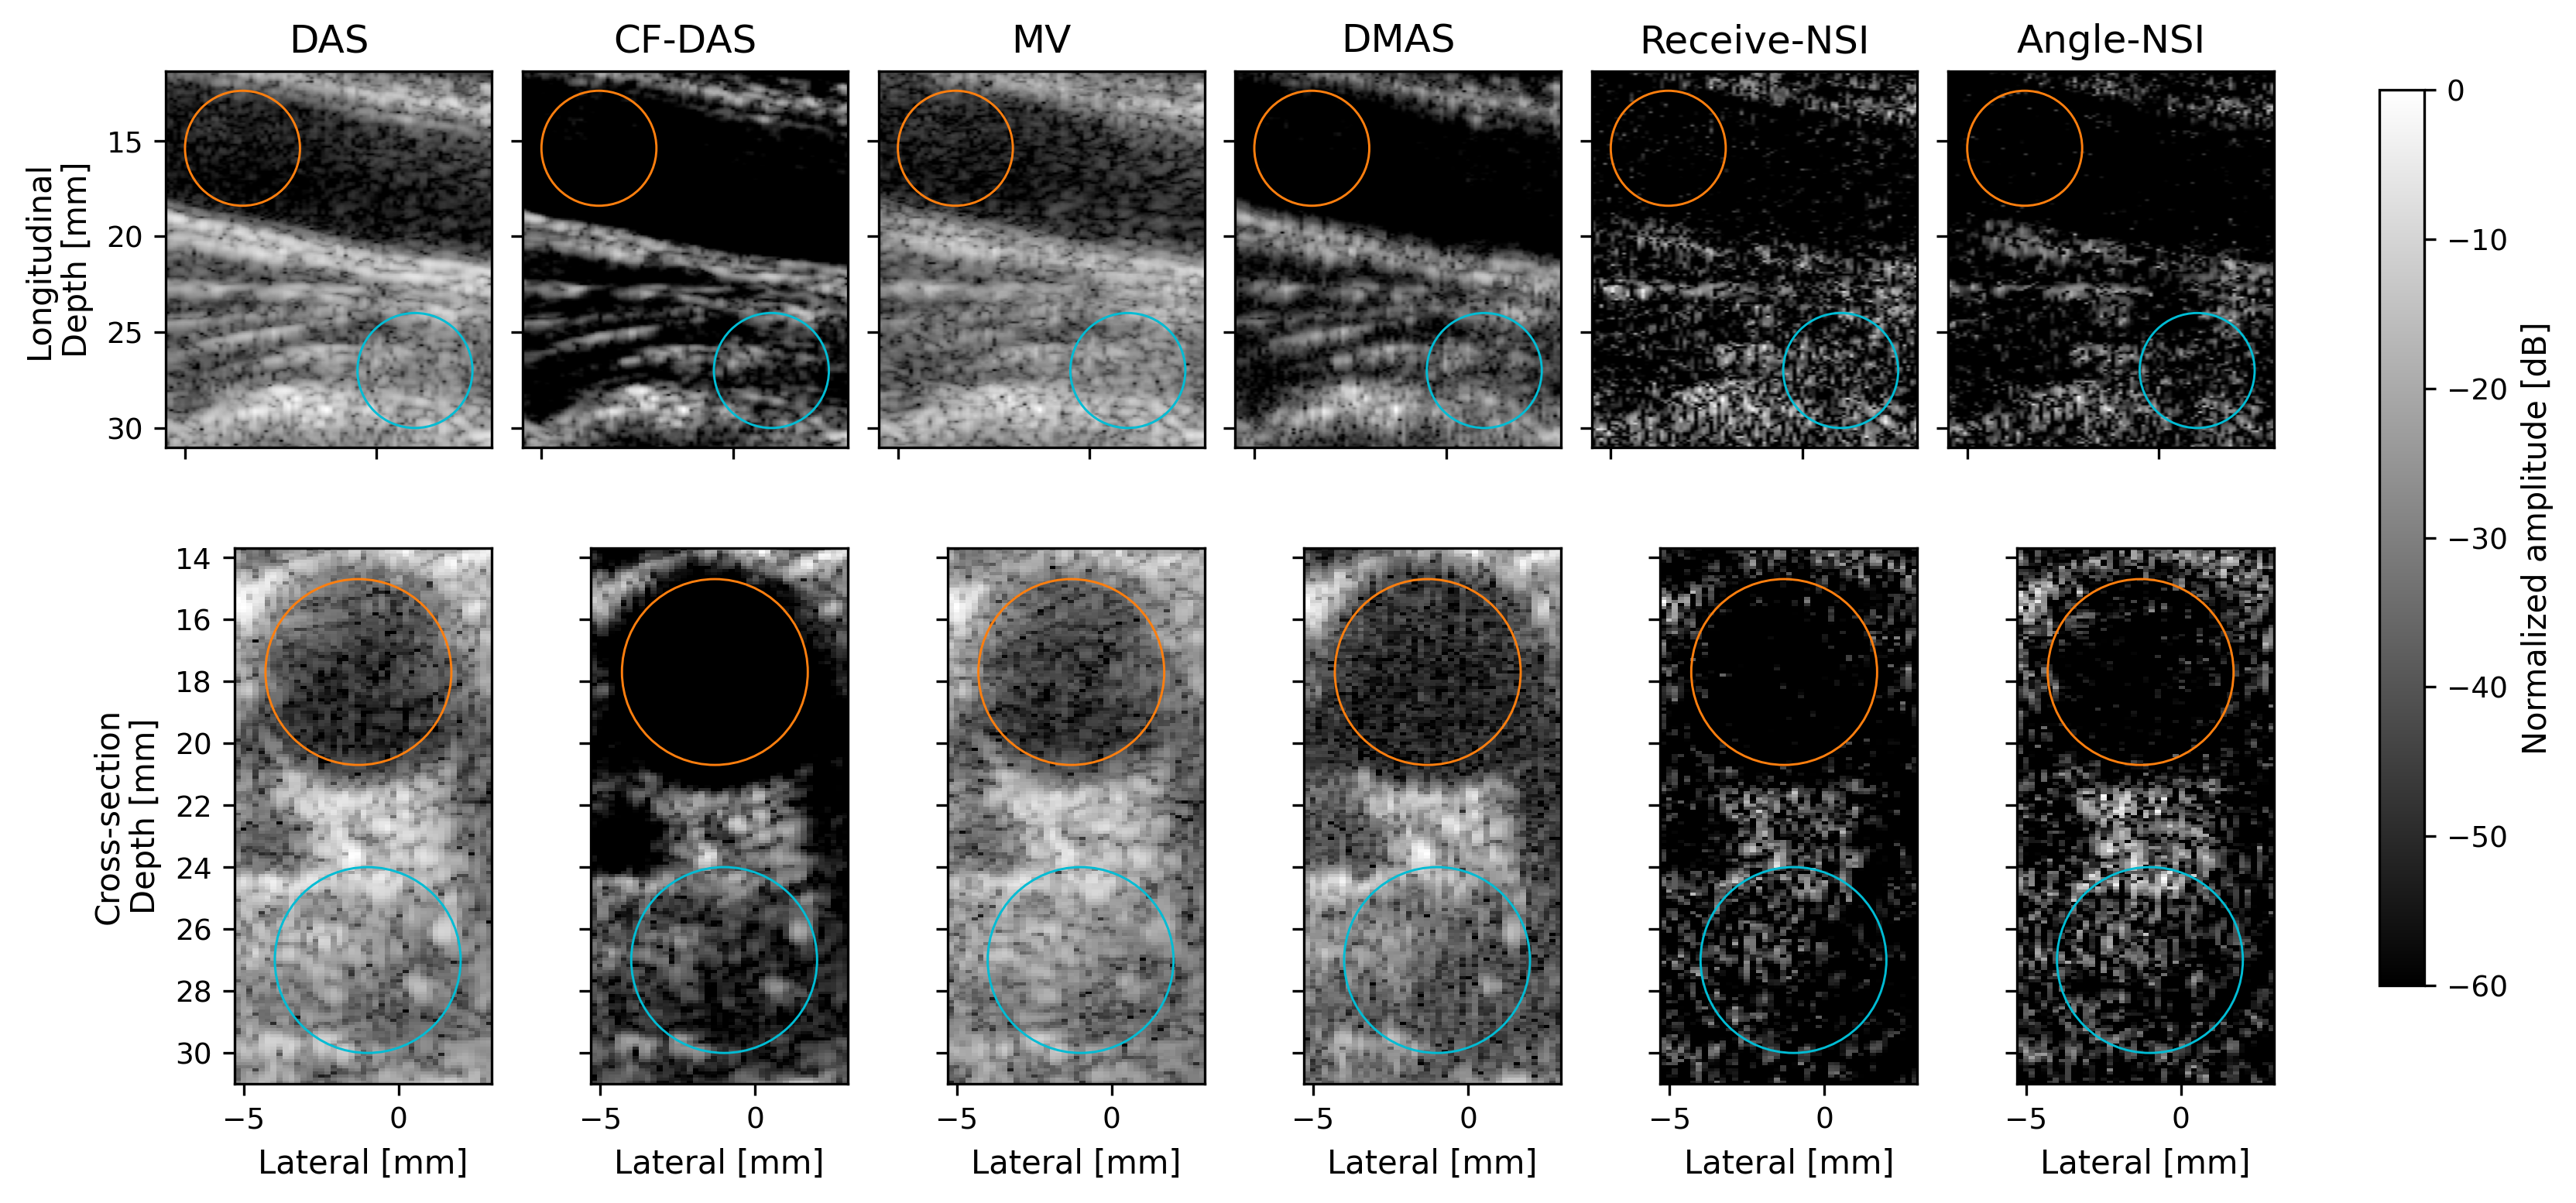
\includegraphics[width=\textwidth]{figures/figure4_carotid_six_method.png}
\caption{\revstart PICMUS longitudinal (top row) and cross-sectional (bottom
row) carotid images for DAS, CF-DAS, MV, DMAS, Receive-NSI and Angle-NSI.
Orange and cyan circles mark the lumen and tissue regions used for gCNR. Each
panel is normalized independently and displayed over 60 dB.\revstop}
\label{fig:carotid}
\end{figure}

\begin{table}[H]
\caption{\revstart Carotid gCNR for the six beamforming methods, calculated in
the lumen and tissue regions shown in Figure~\ref{fig:carotid}.\revstop}
\label{tab:carotid-gcnr}
\centering
\revstart
\begin{tabular}{@{}lrr@{}}
\toprule
Method & Cross-sectional gCNR & Longitudinal gCNR \\
\midrule
DAS & \CarotidCcDasGcnr{} & \CarotidClDasGcnr{} \\
CF-DAS & \CarotidCcCfGcnr{} & \CarotidClCfGcnr{} \\
MV & \CarotidCcMvGcnr{} & \CarotidClMvGcnr{} \\
DMAS & \CarotidCcDmasGcnr{} & \CarotidClDmasGcnr{} \\
Receive-NSI & \CarotidCcReceiveNsiGcnr{} & \CarotidClReceiveNsiGcnr{} \\
Angle-NSI & \CarotidCcAngleNsiGcnr{} & \CarotidClAngleNsiGcnr{} \\
\bottomrule
\end{tabular}
\revstop
\end{table}

\subsection{Robustness and computation}

Angular sampling changed the Angle-NSI PSF non-monotonically. Removing the
$+2^\circ$ transmission widened it from 0.116 mm to 0.147 mm with sign weights
and 0.193 mm after zero-mean recentering. At 10 dB SNR, Angle-NSI width was
$0.122\pm0.005$ mm; a 10$^\circ$ phase-jitter standard deviation increased it
to $0.194\pm0.029$ mm. The complete sweeps are reported in the Supplement.

\revstart End-to-end time scaled approximately with image size, receive
elements and plane waves (Figure~\ref{fig:timing}). In the $128\times256$
reference case, median times were \EndToEndDasTime{},
\EndToEndReceiveNsiTime{} and \EndToEndAngleNsiTime{} ms for DAS, Receive-NSI
and Angle-NSI, confirming the envisioned lower computational cost of Angle-NSI compared to Receive-NSI. The six-method post-delay benchmark exposed the larger MV cost compared to other beamforming techniques, and showed that Angle-NSI is the lightest technique once DAS is excluded. \revstop

\begin{figure}[H]
\centering
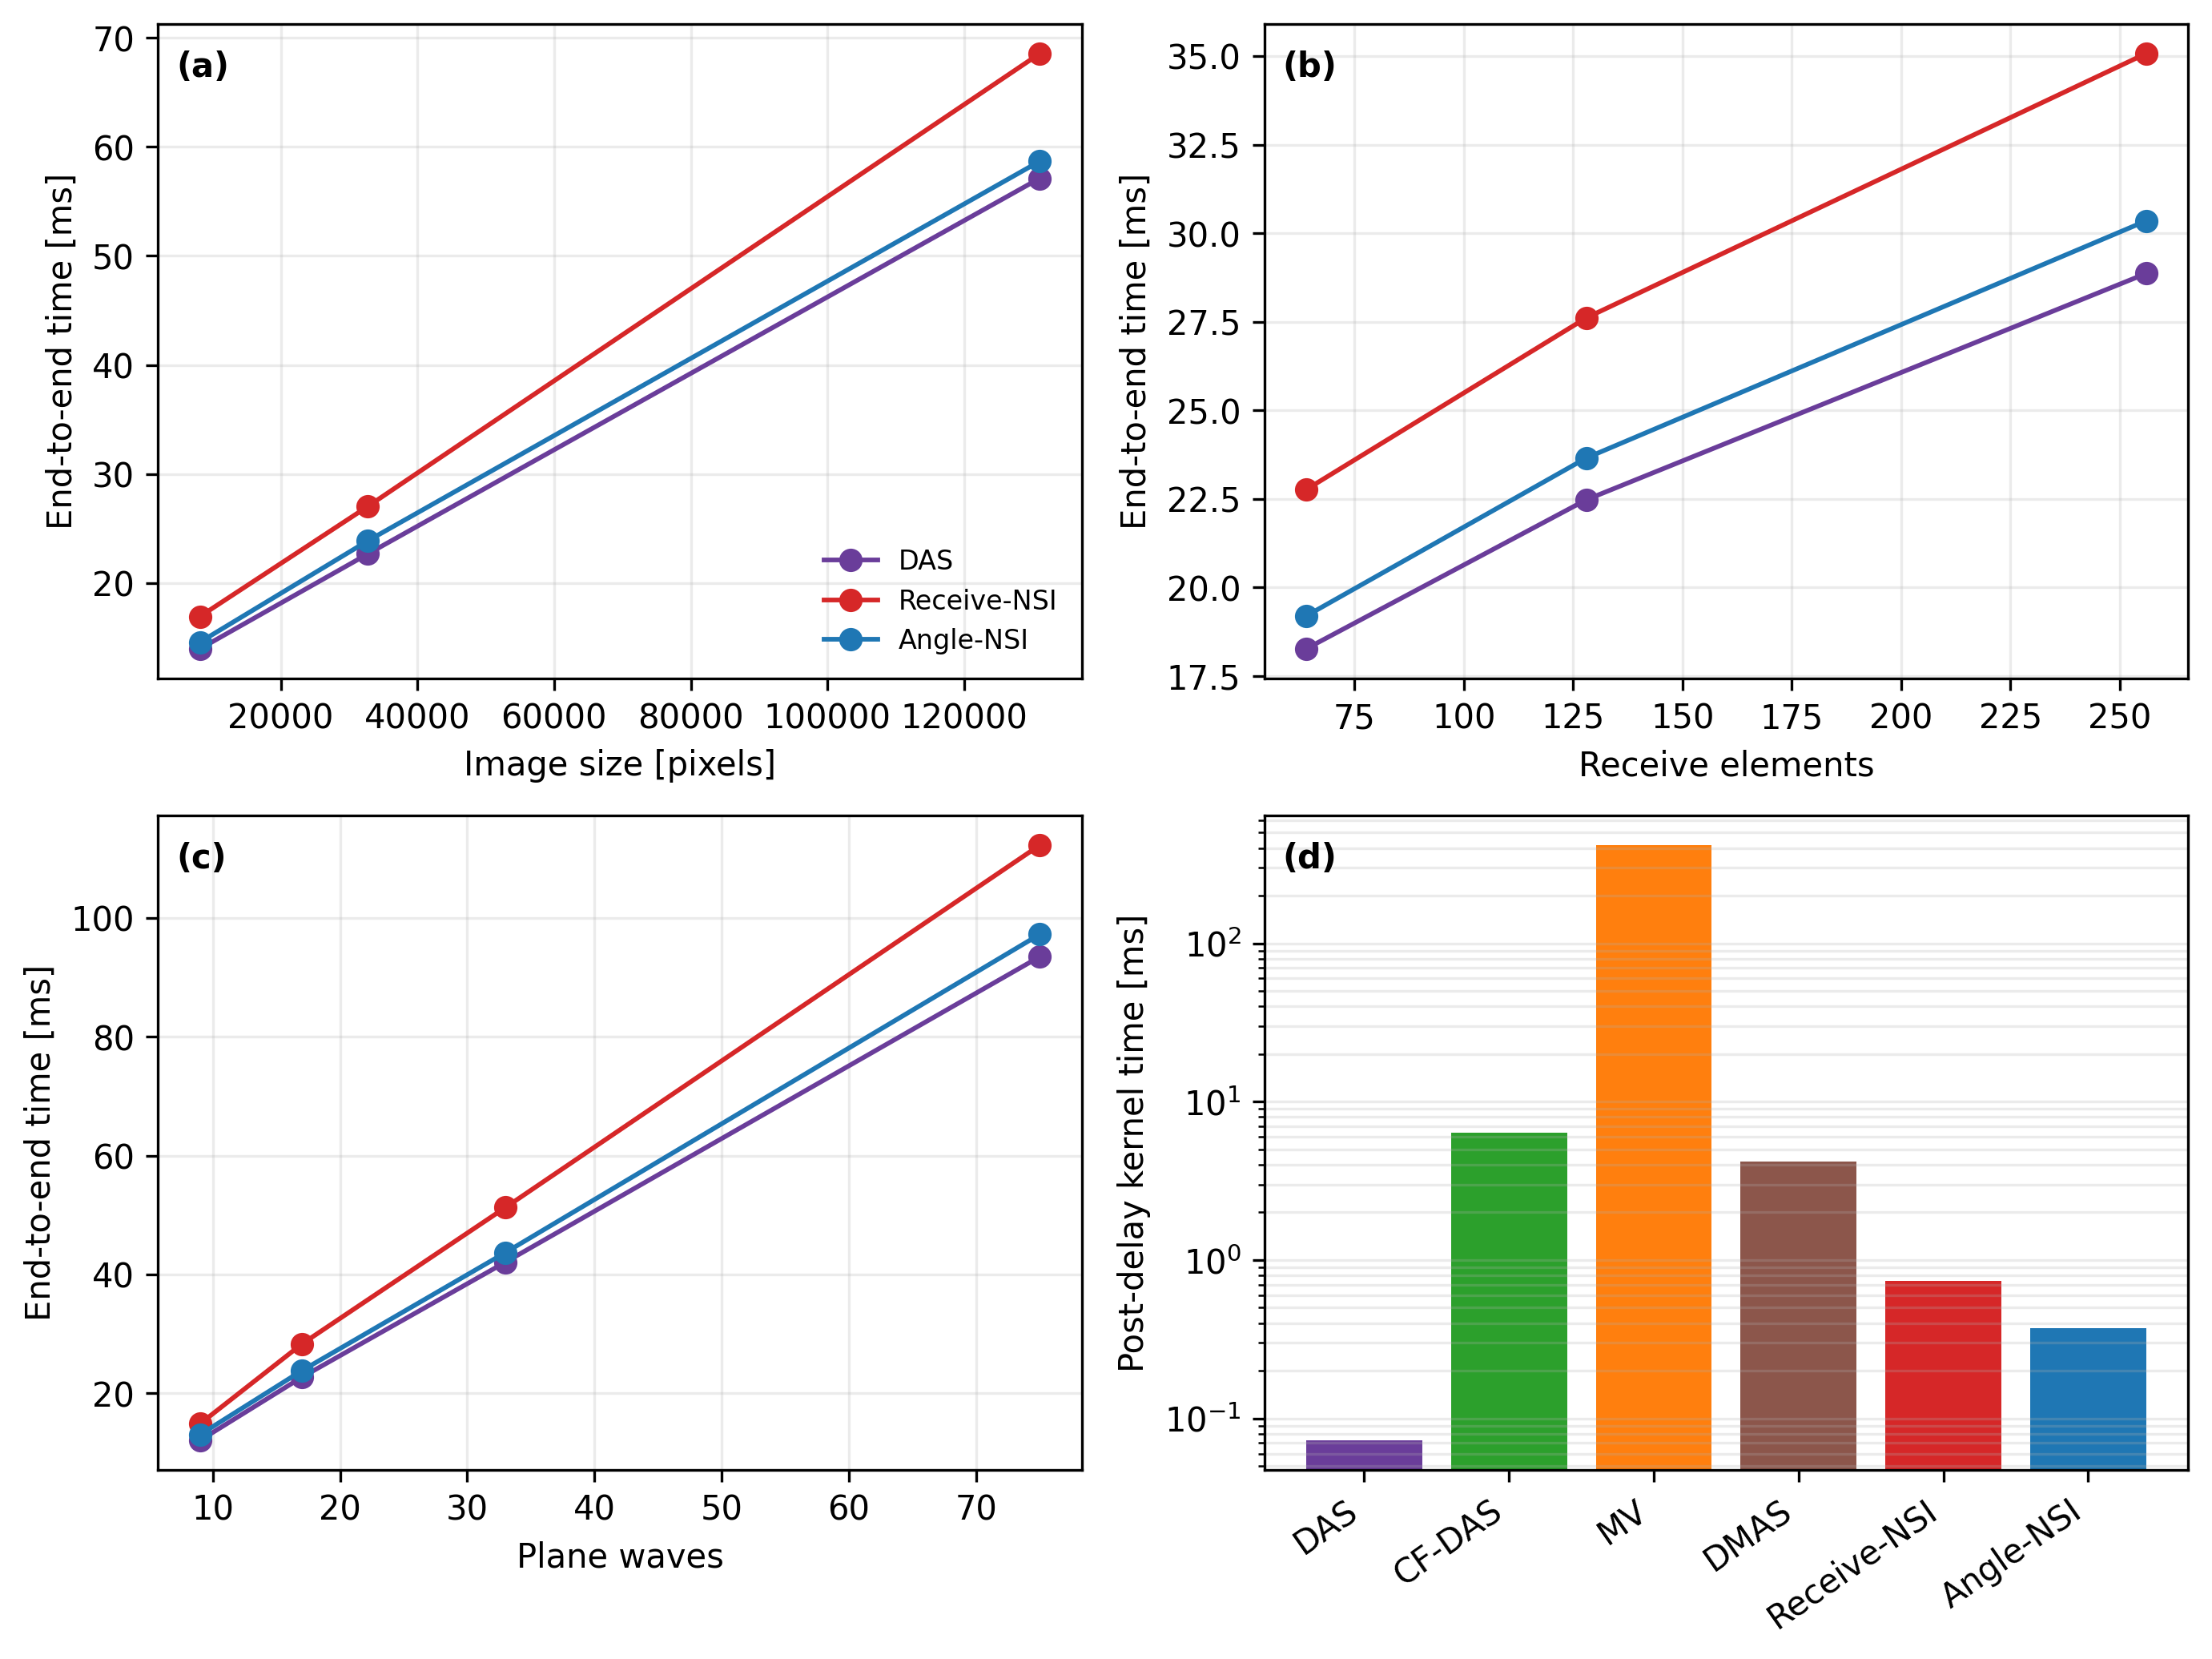
\includegraphics[width=\textwidth]{figures/figure5_computation_benchmark.png}
\caption{\revstart GPU computation benchmark. End-to-end reconstruction time
versus (a) image pixels, (b) receive elements and (c) plane waves for DAS,
Receive-NSI and Angle-NSI. (d) Post-delay kernel time for all six methods on a
logarithmic axis. Points and bars show medians of 50 repetitions.\revstop}
\label{fig:timing}
\end{figure}

\section{Discussion}

The central result is methodological: the NSI framework can use a null formed
across angles after receive beamforming, i.e. it can be adapted from receive
apodization to angular apodization
\citep{rodriguez-molares_angular_2015}. It therefore works from retained
per-angle complex images without channel-data access or custom element
apodization and does not alter delays, interpolation or aperture selection.

The simulations \revstart and experimental resolution phantom study clarify \revstop that the resolution gain is lateral. This is consistent with \revstart Receive-NSI\revstop, which modifies the
receive-aperture pattern but does not shorten the transmitted pulse or increase
its bandwidth \citep{agarwal2019improving}. In the symmetric plane-wave
acquisition studied here, angle-domain weighting similarly reshaped the lateral
angular spectrum while leaving the axial pulse response unchanged. The
\revstart Angle-NSI \revstop lateral width was approximately half that of DAS, \revstart whereas Receive-NSI was considerably narrower. The lateral response gains of NSI compared to DAS are lowered in \textit{in vitro} power Doppler compared to simulations, especially for Receive-NSI. \revstop

\revstart Angle-NSI forms its null across transmit angles; Receive-NSI forms it across receive elements. Their different PSFs, microbubble traces and carotid images confirm that the methods are distinct. \revstop

\revstart The timing study shows the low incremental cost of Angle-NSI under the tested conditions, using per-angle images after ordinary receive beamforming, making it faster than Receive-NSI or other nonlinear beamforming methods. \revstop

The experimental phantom and the carotid results emphasize the resolution--detectability trade-off, \revstart as both NSI
methods decreased gCNR compared to DAS or other nonlinear beamforming methods.\revstop The darker, less speckled images therefore cannot be
interpreted as a general \revstart image-quality \revstop improvement, in accordance with earlier
literature \citep{agarwal2019improving}. This is consistent
with adaptive and post-filtering NSI extensions designed to manage the balance
between narrowing and tissue-image quality
\citep{xu2026regionadaptive,yang2026generalized}. 

The robustness tests identify cancellation across angles as an intrinsic
limitation. Width varied with angle sampling and increased
under phase jitter. After a transmission was removed, zero-mean recentering did
not recover the symmetric response and shifted the peak. \revstart The four
values of the DC offset also changed width, target-to-background level and carotid
distribution metrics.\revstop 

These robustness simulations remain idealized tests with ten perturbation
realizations and discrete grids; sound-speed error, motion and out-of-plane
structures were not tested. The \textit{in vivo} analysis
had only one acquisition per view, while timing used random IQ on
one GPU, and experimental PSFs came from one seven-target phantom.\revstop{} Further validation should extend to several anatomies, motion, and aberration.

\revstart Eventually, the power Doppler study shows that high-resolution Doppler imaging is the most promising use case for Angle-NSI, as it effectively narrows the lateral response of the Doppler signal at a lower computational cost and pipeline complexity compared to Receive-NSI. The use of Angle-NSI for contrast-enhanced and contrast-free Doppler ultrasound, like Receive-NSI \citep{kou2024highresolution}, should be confirmed by further \textit{in vivo} studies. Adapting this new power Doppler technique to enhanced color Doppler imaging, as it has been done with  Receive-NSI \citep{kou_label-free_2025}, could also be explored. \revstop

\section{Conclusion}

In this Note, we investigated \revstart Angle-NSI\revstop, applying envelope subtraction to a null formed across per-angle plane-wave images rather than the channel data. In simulation, \revstart Angle-NSI approximately halved the apparent lateral width. A comprehensive comparison with other beamforming techniques using simulation, a resolution phantom, \textit{in vitro} Doppler data and a carotid acquisition shows that Angle-NSI increases the lateral resolution at the expense of B-Mode detectability, at a low computational cost. Angle-NSI offers simple, low-cost post-processing for high-resolution power Doppler. \revstop

\ack{The author thanks Professor Romain Fleury for hosting his research
activities.}

\funding{This work was supported by EPFL internal funding.}

\roles{Henri Leroy: conceptualization, methodology, software, formal analysis,
investigation, visualization, writing -- original draft, and writing -- review
and editing.}

\data{The MBTrace and PICMUS data sets are publicly available from their
original repositories. Analysis code and result
records are available at
\url{https://github.com/hacheleroy/angle_domain_NSI}.}

\suppdata{\revstart Supplementary figures and tables document the small-angle
model, angular and perturbation sweeps, $c$ sensitivity, MBTrace correspondence,
individual experimental PSF metrics, fixed CF-DAS/MV/DMAS settings and timing controls.
Movies show the unfiltered and SVD-filtered MBTrace sequences for DAS,
Receive-NSI and Angle-NSI.\revstop}

\begingroup
\footnotesize
\bibliographystyle{plainnat}
\bibliography{references}
\endgroup

\end{document}
